\documentclass{article}
\usepackage[a4paper]{geometry}
\pagestyle{empty}
\newgeometry{margin=1cm}
\setlength{\parindent}{0pt}

\usepackage{style}
\usepackage{graphicx}
\usepackage{ragged2e}
\usepackage{hyperref}
\usepackage{tikz}
\tikzstyle{dot}=[circle,fill,inner sep=2pt]

\let\oldhrule\hrule
\renewcommand{\hrule}{\color{LightGray}\oldhrule\color{black}}


\makeatletter
\newcommand{\rubric}[1]{
    \color{MediumGray}

    \section*{\montserratlight \large \MakeUppercase{#1}} 
    \hrule
    \vspace{4mm}
    \raggedright
}

\begin{document}

\begin{minipage}{0.2\textwidth}
  \begin{tikzpicture}
    \clip (0,0) circle (16mm);
    \node[xshift=-2mm, yshift=-2mm] at (0,0) {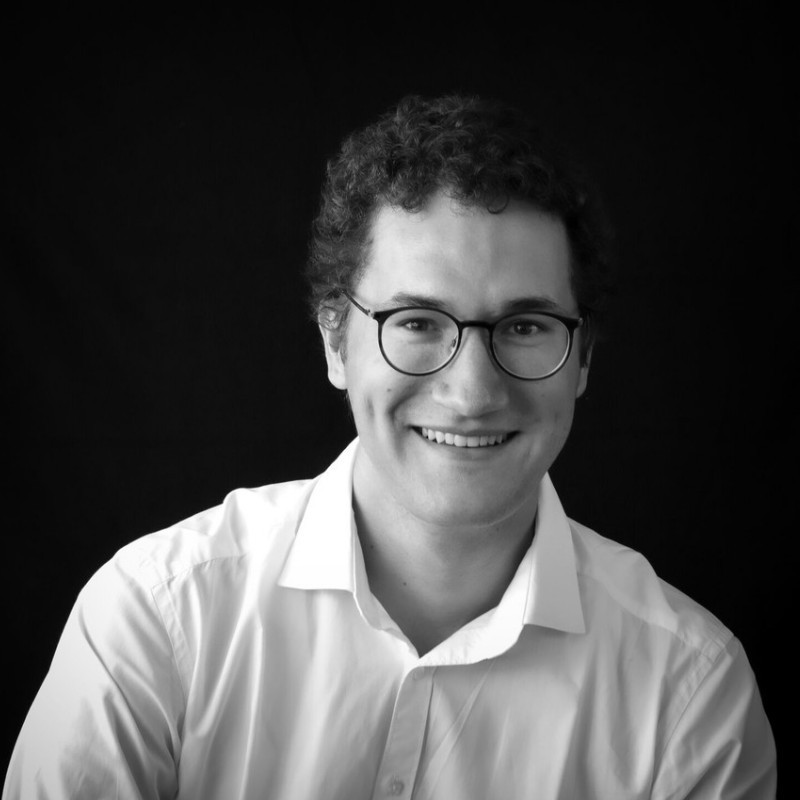
\includegraphics[width=4cm]{arnaud-cv}};
  \end{tikzpicture}

\end{minipage}
\begin{minipage}{0.7\textwidth}
  \centering

  \montserratlight{\Huge ARNAUD  PANNATIER} \\ \vspace{3mm}
  \sc \montserratthin PhD Candidate in Attention-based models
\end{minipage}

\vspace{4mm}
\hrule
\vspace{4mm}
\color{DeepGray}
I am a PhD Candidate in Pr. François Fleuret's Machine Learning group (Idiap Research Institute/EPFL). My main research interests are deep learning architectures and their applications on High-Altitude Wind Nowcasting. \\

\begin{minipage}[t][0.78\textheight][t]{0.3\textwidth}
  \rubric{Education}

  \color{DeepGray}
  \large PhD in Machine Learning \\
  \color{MediumGray} \small
  Innosuisse, with SkySoft ATM \\
  Idiap Research Institute / EPFL \\
  2020 - 2024

  \vspace{4mm}
  \color{DeepGray}
  \large Master in Computer Sciences and Engineering \\
  \color{MediumGray} \small
  Math Faculty, EPFL \\
  2017 - 2020

  \vspace{4mm}
  \color{DeepGray}
  \large Bachelor in Physics \\
  \color{MediumGray} \small
  Physics Faculty, EPFL \\
  2014 - 2017

  \rubric{Languages}
  French: Native speaker \\
  English: Fluent \\
  German: Basic knowledge

  \vfill
  \rubric{Informations}
  Rue des Longs-Prés 40, \\
  3960 Sierre \\

  arnaud.pannatier@idiap.ch \\
  https://arnaudpannatier.ch \\

  \vspace{4mm}

  Born September 20, 1995, in Sion, Valais \\
  Married, two children (born 2022, 2023)

\end{minipage}\hfill
\begin{minipage}[t]{0.65\textwidth}
  \rubric{Publications}
  \small
  A. Pannatier, K. Matoba, F. Fleuret \textbf{Inference from Real-World Sparse Measurements} \textit{under review at International Conference on Learning Representations (ICLR), 2024}
  \vspace{4mm}

  F. Mai, A. Pannatier, F. Fehr, H. Chen, F. Marelli, F. Fleuret, J. Henderson \textbf{HyperMixer: An MLP-based Low Cost Alternative to Transformers.} In \textit{Proceedings of the Annual Meeting of the Association for Computational Linguistics (ACL), 2023.}
  \vspace{4mm}

  A. Pannatier, R. Picatoste, and F. Fleuret. \textbf{Efficient Wind Speed Nowcasting with GPU-Accelerated Nearest Neighbors Algorithm.} In \textit{Proceedings of the SIAM International Conference on Data Mining (SDM), 2022.}
  \vspace{4mm}

  A. Pannatier \textbf{A Control Plane in Time and Space for Locality-Preserving Blockchains} In \textit{Master Thesis, Decentralized Distributed Systems Laboratory (DEDIS), EPFL, 2020} \\
  \textbf{Price: Kudelski Award}

  \rubric{Teaching Experience}

  \color{DeepGray}
  \large Teaching Assistant
  \color{MediumGray} \small
  \begin{itemize}
    \item \color{DeepGray}Advanced Analysis 1-2  \color{MediumGray} Pr. Stubbe, 2016, 2017, 2018
    \item \color{DeepGray}Analysis 2  \color{MediumGray} Pr Buffoni, 2018
    \item \color{DeepGray}Advanced Analysis 3  \color{MediumGray} Pr. Krieger, 2018
    \item \color{DeepGray}Introduction à l'apprentissage automatique  \color{MediumGray} Pr. Liebling, 2020, 2023
    \item \color{DeepGray}Deep Learning  \color{MediumGray} Pr. Fleuret, 2021, 2022
    \item \color{DeepGray}Information, Computation, Communication  \color{MediumGray} Pr. Chappelier, 2020, 2022, 2023
  \end{itemize}

  \vspace{4mm}
  \color{DeepGray}
  \large Substitute Math Teacher \\
  \color{MediumGray} \small
  Lycée Collège de la Planta \\
  2019

  \rubric{Work Experience}

  \color{DeepGray}
  \large Software engineer \\
  \color{MediumGray} \small
  Caelum Fintech SA, Technopôle \\
  2018 - 2020 (Part time)

  \rubric{Hobbies \& Interest}
  \color{DeepGray}
  Hiking \\
  \color{MediumGray} \small
  Hiked from home (VS/CH) to Santiago de Compostella (ES) \\
  2300 km in 83 days (April 2019 - July 2019)
  % \vspace{2mm}

  \color{DeepGray}
  Chess \\
  \color{MediumGray} \small
  Treasurer of the Union Valaisanne des Échecs (UVE-WSB) \\
  Play with "Sion 1" (1st League, previously League B) \\
  Ex-Captain of Chess Team "Valais 2" (2nd league)

\end{minipage}

\end{document}